\documentclass{ctexart}
\usepackage[T1]{fontenc}
\usepackage[a4paper,top=1.5cm,bottom=1.5cm,left=2cm,right=2cm,marginparwidth=1.75cm]{geometry}
\usepackage{mathtools}
\usepackage{tikz}
\usepackage{booktabs}
\usepackage{caption}
\usepackage{outlines}
\usepackage{graphicx}
\usepackage{amsthm}
\usepackage[colorlinks=false, allcolors=blue]{hyperref}
\renewcommand{\tableautorefname}{表}
\DeclarePairedDelimiter{\set}{\{}{\}}
\DeclarePairedDelimiter{\paren}{(}{)}
\graphicspath{ {./images/} }

\title{计算机系统结构第五章作业}
\author{卢雨轩 19071125}
% \date{\today}
\ctexset{
    section = {
        titleformat = \raggedright,
        name = {,},
        number = \chinese{section}、
    },
    paragraph = {
        runin = false
    },
    today = small,
    figurename = 图,
    contentsname = 目录,
    tablename = 表,
}

\begin{document}

\maketitle

\begin{outline}[enumerate]
    \1[5-6] 设16个处理器的编号分别为0、1…、15,用单级互连网络互连时,第9号处理器各与哪一个处理器相连?
    \2 E(X)\\
    9和8相连。
    \2 PM2+3,PM2-1 \\
    9分别和1,7相连。
    \2 Shuffle \\
    9和1相连。
    \2 Butterfly \\
    9(0b1001)和9相连。
    \1[5-11] 在处理器N=8的Omega网络中,若要实现处理器2与所有处理器相连,应怎样设置网络中交叉开关单元的状态?
    \begin{center}
        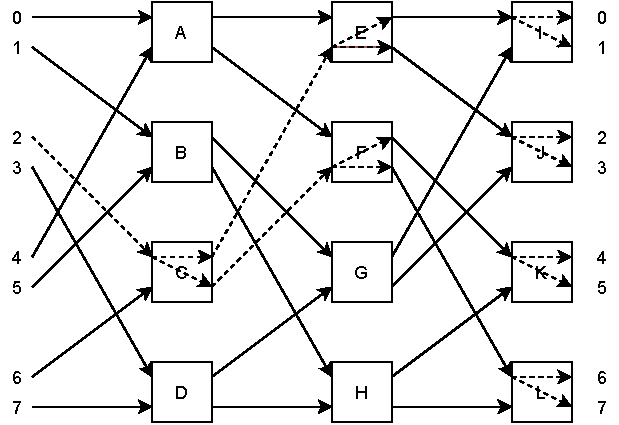
\includegraphics[width=0.8\textwidth]{5-img.pdf}
    \end{center}
    C,I,J,K,L上播;E,F下播。
    
\end{outline}

\end{document}
